% arara: pdflatex: { synctex: yes }
% arara: makeindex: { style: ctuthesis }
%% arara: bibtex


%\listfiles


%\PassOptionsToPackage{cp1250}{inputenc}

% The class takes all the key=value arguments that \ctusetup does,
% and couple more: draft and oneside
\documentclass[twoside]{ctuthesis}

\usepackage{graphicx}
\usepackage{svg}
\usepackage{amsmath}
\usepackage{siunitx}
\usepackage{caption}
\usepackage{subcaption}
\usepackage{placeins}
\usepackage{textgreek}
\usepackage{pdfpages}
\usepackage{bytefield}
\usepackage{tikz-timing}
\usepackage{soul}

\usepackage{float}
\usepackage[defernumbers=true, sorting=none]{biblatex}
\addbibresource{bibliography.bib}


\newcolumntype{?}{!{\vrule width 2pt}}

\usepackage{svg}
\svgsetup{
    inkscape=pdf,
    inkscapeexe={C:/inkscape.exe.lnk -z -C"}
}
\graphicspath{{images/}}

\usepackage[per-mode=symbol,separate-uncertainty=true]{siunitx}


\DeclareSIUnit\bit{b}



\makeatletter
\edef\mytoday{\expandafter\@gobbletwo\the\year\ifnum\month<10 0\fi\the\month\ifnum\day<10 0\fi\the\day}
\makeatother

% LaTeX logo with better kerning in sf bf font
\makeatletter
\newcommand\LaTeX@lmss@bx{L\kern -.33em{\sbox \z@ T\vbox to\ht \z@ {\hbox {\check@mathfonts \fontsize \sf@size \z@ \math@fontsfalse \selectfont A}\vss }}\kern -.15em\TeX}
\DeclareRobustCommand\myLaTeX{%
	\ifcsname LaTeX@\f@family @\f@series\endcsname
		\csname LaTeX@\f@family @\f@series\endcsname
	\else
		\LaTeX
	\fi
}

\ctusetup{
%	preprint = {\ctuverlog \\ ctuman \mytoday},
	mainlanguage = english,
	titlelanguage = english,
	otherlanguages = {english},
	title-czech = {Vyčítací systém pro FastIC+},
	title-english = {FastIC+ readout system},
	doctype-english = {Diploma Thesis},
	xfaculty = F3,
        xdoctype = M,
	department-english = {Department of Microelectronics},
%	department-english = {Department of Mathematics},
	author = {Bc. Vojtěch Vosáhlo},
	supervisor = {Ing. Vít Záhlava, CSc.},
        fieldofstudy-english = {Electronics},
%	supervisor-address = {Ústav X, \\ Uliční 5, \\ Praha 99},
	keywords-czech = {DPS, Internet Věcí, brána, BLE, Zigbee},
	keywords-english = {PCB, Internet of Things, gateway, BLE, Zigbee},
	day = 25,
	month = 5,
	year = 2023,
%	list-of-figures = false,
%	list-of-tables = false,
%	monochrome = true,
%	savetoner = true,
	pkg-listings = true,
        pkg-makeidx = true,
	ctulstbg = none,
%	layout-short = true,
}

\ctuprocess

% Theorem declarations, this is the reasonable default, anybody can do what they wish.
% If you prefer theorems in italics rather than slanted, use \theoremstyle{plainit}
\theoremstyle{plain}
\newtheorem{theorem}{Theorem}[chapter]
\newtheorem{corollary}[theorem]{Corollary}
\newtheorem{lemma}[theorem]{Lemma}
\newtheorem{proposition}[theorem]{Proposition}

\theoremstyle{definition}
\newtheorem{definition}[theorem]{Definition}
\newtheorem{example}[theorem]{Example}
\newtheorem{conjecture}[theorem]{Conjecture}

\theoremstyle{note}
\newtheorem*{remark*}{Remark}
\newtheorem{remark}[theorem]{Remark}

% Marginpars used as navigation aids.
\usepackage{mparhack}
\usepackage{makecell}

\newcommand\indexmp[1]{{\sffamily\bfseries#1}}

\ExplSyntaxOn
\cs_new:Nn \ctuman_domarginpar:n {
	\marginpar
	[ \raggedleft \footnotesize \sffamily #1 ]
	{ \raggedright \footnotesize \sffamily #1 }
}
\cs_generate_variant:Nn \ctuman_domarginpar:n { x }
\DeclareDocumentCommand \ctump { m } {
	\clist_set:Nn \ctuman_temp_clist { #1 }
	\ctuman_domarginpar:x { \clist_use:Nnnn \ctuman_temp_clist { \\ } { \\ } { \\ } }
	\clist_map_inline:Nn \ctuman_temp_clist { \index{##1|indexmp} }
	\ignorespaces
}
\ExplSyntaxOff

\sisetup{locale = UK}

% Abstract in Czech
\begin{abstract-czech}
Tato práce se zabývá návrhem elektronického systému určeného k vyčítání dat z integrovaných obvodů FastIC+ vyvíjených v rámci CERN. Prvně nastiňue vlastnosti zmíněných ASIC a jejich účel. Následně detailně popisuje návrh elektroniky a firmware zařízení. V neposlední řadě popisuje také návrh uživatelského rozhraní. 
\end{abstract-czech}

% Abstract in English
\begin{abstract-english}
----
\end{abstract-english}

% Acknowledgements / Podekovani
\begin{thanks}
----
\end{thanks}

% Declaration / Prohlaseni
\begin{declaration}
Prohlašuji, že jsem předloženou práci vypracoval samostatně, a že jsem uvedl veškerou použitou literaturu.

\medskip

V Praze,  \ctufield{day}.~\monthinlanguage{title}~\ctufield{year}

\vspace*{2cm}

I declare that this work is all my own work and I have cited all sources I have
used in the bibliography.

\medskip

Prague, \monthinlanguage{second} \ctufield{day}, \ctufield{year}
\end{declaration}

\usepackage{url}

\usepackage{tabularx,array}

\usepackage{mathtools,amssymb}
\usepackage{threeparttable}[para,online,flushleft]
\usepackage{makecell}


\usepackage{float}
\floatstyle{plaintop}
\restylefloat{table}

% A savebox for typesetting listings in the titles
\newsavebox{\myboxa}

%\newcommand*\symbO{$\color{red}\bowtie$}
\newcommand*\symbO{\raisebox{0.5\height}{\scalebox{0.7}{\color{red}${\vartriangleright}\mkern-6mu{\vartriangleleft}$}}}
\newcommand*\symbM{\raisebox{0.5\height}{\scalebox{0.7}{\color{red}${\blacktriangleright}\mkern-6mu{\blacktriangleleft}$}}}
\newcommand*\itemO{\item\leavevmode\kern-0.33em\symbO}
\newcommand*\itemM{\item\leavevmode\kern-0.33em\symbM}



\begin{document}

% We actually don't want inline listings to have a background color
\renewcommand \ctulstsep {0pt}

% \ctuclsname for typesetting the class' name
\newcommand\ctuclsname{\leavevmode\unhcopy\ctuclsnamebox}
\newsavebox\ctuclsnamebox
\begin{lrbox}{\ctuclsnamebox}
\ctulst!ctuthesis!
\end{lrbox}

\maketitle


\newpage
\begingroup
\color{black}
\tableofcontents
\endgroup

\pagebreak

\chapter{Introduction}
In order to enhance the time measurement of the ToA and ToT analog pulses, FastIC+ has added a picosecond TDC for digitizing the pulses on the chip itself. This, in turn, has necessitated the need for a high-speed communication channel capable of transferring the resulting data stream. The Aurora 64B/66B protocol was chosen for its sufficient speed and easy interfacing with FPGAs.


\chapter{FastIC+}
The FastIC+ is an 8-channel front-end for photo detectors such as SiPM, PMT or MCP, capable of precisely
measuring the Time-of-Arrival (ToA) and energy of photons hitting the detector from the Time-over-Treshold (ToT). 

\section{Detection}
\label{sec:fastic:detection}
The detection part of the chip implements current mode front-ends capable of working with both positive and negative polarity sensors with dynamic range of \SI{5}{\micro\ampere} to \SI{20}{\milli\ampere} and capacitance range of \SI{10}{\pico\farad} to \SI{1}{\nano\farad}. The eight channels can either operate independently or in a summation mode and can be highly configured to suffice demanding user needs. Several triggering schemes are available for discriminating the photon impacts by their energy aswell as external trigger input and trigger output to allow synchronization of multiple chips. Three different measurement modes, 
\begin{itemize}
    \item ToA (Non linear ToT),
    \item Energy (from ToT),
    \item Hybrid (ToA + Energy),
\end{itemize}
are present to allow the user to optimize for measurement of ToA, ToT or both. The maximum detection rate of the impacts is approximately \SI{2}{\mega\hertz} in the linear mode and \SI{50}{\mega\hertz} in non-linear mode. A \SI{40}{\mega\hertz} low jitter reference clock is required for the chip to operate.


\section{Digitizing}
The measured ToA and ToT are outputted separately for each channel as a digital pulse, where the beginning of the pulse marks the ToA of the photon and the length of the pulse encodes the energy (ToT). These channels are exposed to the user and can be used for photon detection.

However in order to enhance the time measurement of the ToA and ToT pulses and offload this processing from the user, a \SI{25}{\pico\second} time bin TDC for digitizing the pulses directly on the chip has been implemented. This, in turn, has necessitated the need for a high-speed communication channel capable of transferring the resulting digital data stream. The Aurora 64B/66B protocol was chosen for its sufficient speed and easy interfacing with FPGAs. The FastIC+ itself implements a simplified Aurora transmitter with one simplex lane capable of transmission at speeds from \SI{80}{\mega\bit\per\second} to \SI{1.28}{\giga\bit\per\second}.

\section{Configuration and testing}
An I2C interface has been implemented alongside the Aurora bus to allow for easy configuration of the chip parameters. This interface can run at speeds up to \SI{1}{\mega\hertz} and can be shared between multiple FastIC+ chips. 

For testing purposes, four debug pins are exposed to read out the state of the internal state machine. If not used for debugging, they can be utilized for configuration of the I2C address. 

\chapter{Aurora protocol}
Aurora 64B/66B is a link-layer, point-to-point protocol that enables high-speed data transfers between two Aurora partners. The Aurora channel, established between the partners, can comprise one or more simplex or full-duplex lanes. Data frames are transmitted in 66-bit blocks, consisting of a two-bit synchronization preamble and 64 bits of data. The channel is shared for both data and control messages. 
\section{Frame notation}
Frame notation and bit order adopted from the Aurora specification \cite{auroraSpec} citace will be used in this document. In this notation the leftmost bit is the one transmitted first onto the bus and is considered the most significant in the block. The rightmost bit is LSB. An example of a block notation can be seen in Figure \ref{fig:blockExample}.
\\
\FloatBarrier
\begin{figure}[htpb]
    \begin{center}
        \begin{bytefield}[endianness=little,bitwidth=0.8em]{32}
            \bitheader{0,1,2,9,10,17,18,25,26,33} \\
            \bitbox{1}{\texttt{\footnotesize 0}} & \bitbox{1}{\texttt{\footnotesize 1}} & \bitbox{8}{\texttt{\footnotesize MSB}} &
            \bitbox{8}{} & \bitbox{8}{} & \bitbox{8}{}\\[3ex]
            \hfill
            \bitheader[lsb=34]{34,41,42,49,50,57,58,65} \\
            \hfill
            \bitbox{8}{} & \bitbox{8}{} & \bitbox{8}{} & \bitbox{8}{\texttt{\footnotesize LSB}}
        \end{bytefield}
        \caption{Example Aurora block structure}
        \label{fig:blockExample}
    \end{center}
\end{figure}
%
\section{Encoding}
As previously mentioned, the Aurora protocol utilizes the commonly used 64B/66B encoding. This encoding scheme converts 64 bits of data into a 66-bit block by appending a two-bit preamble. The \verb|01| preamble signifies that the block contains 8 octets of data and is therefore called a \emph{Data block}. If the preamble is \verb|10|, the block is recognized as \emph{Control block} with the most significant octet in the block being a \emph{BTF} (Block Type Field). The remaining 7 octets are data. Preambles \verb|00| and \verb|11| are interpreted as errors.
\newline\newline
FastIC+ is capable of transmitting the \emph{Data block} and four of the \emph{Control block} types:
\begin{itemize}
    \item \emph{Separator-7} block indicated by the \emph{BTF} value \verb|0xE1|,
    \item \emph{Separator} block indicated by the \emph{BTF} value \verb|0x1E|,
    \item \emph{User K-Block} with \emph{BTF} value indicating the ID of the block (see \ref{sec:kblock}),
    \item \emph{Idle} block indicated by the \emph{BTF} value \verb|0x78|.
\end{itemize}

\subsection{Data block}
A \emph{Data block}, shown in Figure \ref{fig:data}, consists of eight octets of raw data. Data blocks are transmitted only when eight or more octets of data are available. For smaller packets, the \emph{Separator-7} and \emph{Separator} blocks are used.
\\
\FloatBarrier
\begin{figure}[!htpb]
    \begin{center}
        \begin{bytefield}[endianness=little,bitwidth=0.8em]{32}
            \bitheader{0,1,2,9,10,17,18,25,26,33} \\
            \bitbox{1}{\texttt{\footnotesize 0}} & \bitbox{1}{\texttt{\footnotesize 1}} & \bitbox{8}{\texttt{\footnotesize D7}} &
            \bitbox{8}{\texttt{\footnotesize D6}} & \bitbox{8}{\texttt{\footnotesize D5}} & \bitbox{8}{\texttt{\footnotesize D4}}\\[3ex]
            \hfill
            \bitheader[lsb=34]{34,41,42,49,50,57,58,65} \\
            \hfill
            \bitbox{8}{\footnotesize D3} & \bitbox{8}{\texttt{\footnotesize D2}} & \bitbox{8}{\texttt{\footnotesize D1}} & \bitbox{8}{\texttt{\footnotesize D0}}
        \end{bytefield}
        \caption{Data block structure}
        \label{fig:data}
    \end{center}
\end{figure}

\subsection{Separator-7 block}
A \emph{Separator-7 block} is transmitted when only seven octets of data remain to be sent over the interface. The block consists of the \emph{BTF} indicating the  \emph{Separator-7} type and seven valid octets of data as shown in Figure \ref{fig:sep7}.
\\
\FloatBarrier
\begin{figure}[!htpb]
    \begin{center}
        \begin{bytefield}[endianness=little,bitwidth=0.8em]{32}
            \bitheader{0,1,2,9,10,17,18,25,26,33} \\
            \bitbox{1}{\texttt{\footnotesize 1}} & \bitbox{1}{\texttt{\footnotesize 0}} & \bitbox{8}{\texttt{\footnotesize 0xE1}} &
            \bitbox{8}{\texttt{\footnotesize D6}} & \bitbox{8}{\texttt{\footnotesize D5}} & \bitbox{8}{\texttt{\footnotesize D4}}\\[3ex]
            \hfill
            \bitheader[lsb=34]{34,41,42,49,50,57,58,65} \\
            \hfill
            \bitbox{8}{\texttt{\footnotesize D3}} & \bitbox{8}{\texttt{\footnotesize D2}} & \bitbox{8}{\texttt{\footnotesize D1}} & \bitbox{8}{\texttt{\footnotesize D0}}
        \end{bytefield}
        \caption{Separator-7 block structure}
        \label{fig:sep7}
    \end{center}
\end{figure}
\newpage
\subsection{Separator block}
A \emph{Separator block} is transmitted when 0-6 octets of data remain to be sent. The block, shown in Figure \ref{fig:sep}, consists of the \emph{BTF} indicating the \emph{Separator} type and a field indicating the number of valid data octets. The order of the valid octets is from LSB to MSB. 
\\
\FloatBarrier
\begin{figure}[!htpb]
    \begin{center}
        \begin{bytefield}[endianness=little,bitwidth=0.8em]{32}
            \bitheader{0,1,2,9,10,17,18,25,26,33} \\
            \bitbox{1}{\texttt{\footnotesize 1}} & \bitbox{1}{\texttt{\footnotesize 0}} & \bitbox{8}{\texttt{\footnotesize 0x1E}} &
            \bitbox{8}{\texttt{\footnotesize VALID OCTETS}} & \bitbox{8}{\texttt{\footnotesize D5}} & \bitbox{8}{\texttt{\footnotesize D4}}\\[3ex]
            \hfill
            \bitheader[lsb=34]{34,41,42,49,50,57,58,65} \\
            \hfill
            \bitbox{8}{\texttt{\footnotesize D3}} & \bitbox{8}{\texttt{\footnotesize D2}} & \bitbox{8}{\texttt{\footnotesize D1}} & \bitbox{8}{\texttt{\footnotesize D0}}
        \end{bytefield}
        \caption{Separator block structure}
        \label{fig:sep}
    \end{center}
\end{figure}

\subsection{User K-block}
\label{sec:kblock}
\emph{User K-Blocks} are provided by the Aurora specification to allow the user application to send specific control messages separately from the data. Figure \ref{fig:kblock} shows the \emph{K-Block} comprising the \emph{BTF} and seven data octets. There are nine \emph{K-Blocks} available with IDs 0 to 8, corresponding to \emph{BTFs} \verb|0xD2|, \verb|0x99|, \verb|0x55|, \verb|0xB4|, \verb|0xCC|, \verb|0x66|, \verb|0x33|, \verb|0x4B| and \verb|0x87|, respectively.
\\
\FloatBarrier
\begin{figure}[!htpb]
    \begin{center}
        \begin{bytefield}[endianness=little,bitwidth=0.8em]{32}
            \bitheader{0,1,2,9,10,17,18,25,26,33} \\
            \bitbox{1}{\texttt{\footnotesize 1}} & \bitbox{1}{\texttt{\footnotesize 0}} & \bitbox{8}{\texttt{\footnotesize BTF}} &
            \bitbox{8}{\texttt{\footnotesize D6}} & \bitbox{8}{\texttt{\footnotesize D5}} & \bitbox{8}{\texttt{\footnotesize D4}}\\[3ex]
            \hfill
            \bitheader[lsb=34]{34,41,42,49,50,57,58,65} \\
            \hfill
            \bitbox{8}{\texttt{\footnotesize D3}} & \bitbox{8}{\texttt{\footnotesize D2}} & \bitbox{8}{\texttt{\footnotesize D1}} & \bitbox{8}{\texttt{\footnotesize D0}}
        \end{bytefield}
        \caption{User K-Block structure}
        \label{fig:kblock}
    \end{center}
\end{figure}
\newpage
\subsection{Idle block}
Figure \ref{fig:idle} shows a structure of an \emph{Idle block}. When no data is available for transmission, \emph{Idle} blocks are transmitted instead to maintain the receivers ability to remain in sync and recover the data clock.
\\
\FloatBarrier
\begin{figure}[h!]
    \begin{center}
        \begin{bytefield}[endianness=little,bitwidth=0.8em]{32}
            \bitheader{0,1,2,9,10,11,12,13,14,15,16,17,18} \\
            \bitbox{1}{\texttt{\footnotesize 1}} & \bitbox{1}{\texttt{\footnotesize 0}} & \bitbox{8}{\texttt{\footnotesize 0x78}} &
            \bitbox{1}{\texttt{\tiny CC}} & \bitbox{1}{\texttt{\tiny CB}} & \bitbox{1}{\texttt{\tiny NR}} & \bitbox{1}{\texttt{\tiny SA}} & \bitbox{1}{\texttt{\footnotesize 0}} & \bitbox{1}{\texttt{\footnotesize 0}} & \bitbox{1}{\texttt{\footnotesize 0}} & \bitbox{1}{\texttt{\footnotesize 0}} & \bitbox[ltb]{16}{\texttt{\footnotesize Don't care}}\\[3ex]
            \hfill
            \bitheader[lsb=34]{65} \\
            \hfill
            \bitbox[tbr]{32}{\texttt{\footnotesize Don't care}}
        \end{bytefield}
    \end{center}
    \caption{Idle block structure}
    \label{fig:idle}
\end{figure}
\FloatBarrier
%
%
\noindent
The \emph{Idle block} contains four flag bits determining the type of the block:
\begin{itemize}
    \item \verb|CC| bit indicating that the block is \emph{Clock Compensation} idle,
    \item \verb|CB| bit indicating that the block is \emph{Channel Bonding} idle,
    \item \verb|NR| bit indicating that the block is a \emph{Not Ready} idle,
    \item \verb|SA| bit indicating that the receivers obey the \emph{Strict Alignment} rules.
\end{itemize}
As the Aurora interface in the FastIC+ is simplex and doesn't implement the functionality described above, all the flag bits in the block are set to zero thus only a \emph{Regular Idle} block is being transmitted. 

\section{Scrambling}
Whenever either \emph{Data Block} or \emph{Control Block} is transmitted, the eight octets in the block have to be scrambled with the polynomial shown in Equation \ref{eq:scrambler}. Note that the two bit preamble must never be scrambled.
\begin{equation}
    P(x) = 1 + x^{39} + x^{58}
    \label{eq:scrambler}
\end{equation}
\chapter{FastIC+ packet structure}
%
As mentioned in section \ref{sec:fastic_digitizing}, the ASIC encodes the timing and other information into a format suitable for transmission. The structure of these packets is described
\section{Data packet}
%
Each detection event on each channel of the FastIC+ is represented by a 48 bit data packet containing the digitized \emph{ToA} and \emph{ToT} values. The stream of packets is then encoded into Aurora data blocks. A structure of the packet is depicted in Figure \ref{fig:packet}.
\\
\FloatBarrier
\begin{figure}[tph!]
    \begin{center}
        \begin{bytefield}[endianness=little,bitwidth=4em, bitheight=1.2em]{8}
            \bitheader{0,1,2,3,4,5,6,7} \\
            \bitbox{4}{\texttt{\footnotesize CHANNEL}} & \bitbox{2}{\texttt{\footnotesize TYPE}} & \bitbox[ltr]{2}{} \\
            \bitbox[lr]{8}{\texttt{\footnotesize TIMESTAMP}} \\
            \bitbox[lr]{8}{\texttt{\footnotesize (22 bits)}} \\
            \bitbox[lrb]{4}{} & \bitbox[lrt]{4}{} \\
            \bitbox[lr]{8}{\texttt{\footnotesize PULSE WIDTH (14 bits)}}  \\
            \bitbox[lrb]{2}{} & \bitbox{1}{\texttt{\footnotesize DBG}} & \bitbox{1}{\texttt{\footnotesize CHP}} & \bitbox{1}{\texttt{\footnotesize TYP}} &
            \bitbox{1}{\texttt{\footnotesize TSP}} & \bitbox{1}{\texttt{\footnotesize PWP}} & \bitbox{1}{\texttt{\footnotesize PAR}} 
        \end{bytefield}
    \end{center}
    \caption{FastIC+ data packet structure}
    \label{fig:packet}
\end{figure}
%
\noindent The \verb|CHANNEL| field specifies the number of the channel that the event was detected on (0-7) or the trigger channel (8). The \verb|TYPE| field indicates the packet type where the following types are recognized:
\begin{itemize}
    \item \emph{ToA + non-linear ToT} type represented by the value \verb|0b00|,
    \item \emph{ToA only} type represented by the value \verb|0b01|,
    \item \emph{Linear ToT only} type represented by the value \verb|0b10|,
    \item \emph{ToA + linear ToT} type represented by the value \verb|0b11|.
\end{itemize}
%
\verb|TIMESTAMP| and \verb|PULSE WIDTH| fields contain the digitized ToA and ToT values. \verb|DBG| is a flag used in debug mode. The rest of the bits are even parity bits, namely:
\begin{itemize}
    \item \verb|CHP| parity bit of the \verb|CHANNEL| field,
    \item \verb|TYP| parity bit of the \verb|TYPE| field,
    \item \verb|TSP| parity bit of the \verb|TIMESTAMP| field,
    \item \verb|PWP| parity bit of the \verb|PULSE WIDTH| field,
    \item and the overall parity bit \verb|PAR| computed from all fields.
\end{itemize}

\section{Statistics packet}
In addition to the data packets, FastIC+ also periodically transmits a statistics packet that contains basic information about the past events. Structure of the packet is shown in Figure \ref{fig:statpacket}. This packet is sent onto the Aurora bus in two \emph{K-Blocks} due to the packet size being bigger than the \emph{K-Block} capacity. The first 56 bits are sent in a block with the \emph{BTF} of \verb|0x99|, the rest is sent in a second block with the \emph{BTF} of \verb|0x55|.
\\
\FloatBarrier
\begin{figure}[tph!]
    \begin{center}
        \begin{bytefield}[endianness=little,bitwidth=4em, bitheight=1.2em]{8}
            \bitheader{0-7} \\
            \bitbox[lrt]{8}{\texttt{\footnotesize FIFO DROP}}\\
            \bitbox[lr]{8}{\texttt{\footnotesize (20 bits)}}\\
            \bitbox[lrb]{4}{} & \bitbox[lrt]{4}{}\\
            \bitbox[lr]{8}{\texttt{\footnotesize PWIDTH DROP}}\\
            \bitbox[lrb]{8}{\texttt{\footnotesize (20 bits)}}\\
            \bitbox[lrt]{8}{\texttt{\footnotesize DCOUNT DROP}}\\
            \bitbox[lr]{8}{\texttt{(\footnotesize 20 bits)}}\\
            \bitbox[lrb]{4}{} & \bitbox[lrt]{4}{}\\
            \bitbox[lr]{8}{\texttt{\footnotesize TRIGGER DROP}}\\
            \bitbox[lrb]{8}{\texttt{\footnotesize (20 bits)}}\\
            \bitbox[lrt]{8}{\texttt{\footnotesize PULSE ERROR}}\\
            \bitbox[lrb]{8}{\texttt{\footnotesize (16 bits)}}
        \end{bytefield}
    \end{center}
    \caption{FastIC+ statistics packet structure}
    \label{fig:statpacket}
\end{figure}
%
\noindent The packet consists of the following fields:
\begin{itemize}
\item \verb|FIFO DROP| field containing a number of events dropped in the FIFO buffer.
\item \verb|PWIDTH DROP| field containing a number of events dropped due to the pulse width being outside of the specified range.
\item \verb|DCOUNT DROP| field holding the value of dark counts. This field is valid only if \emph{High-Energy Resolution} mode and \emph{Bandwidth optimization} is enabled. 
\item \verb|TRIGGER DROP| field holding the number of packets dropped due to external trigger pulse not being validated. 
\item \verb|PULSE ERROR| field being a malformed pulse counter. Malformed pulse is detected when two consecutive edges are read by the TDC. This may occur due to the limitation of one leading+falling edge per clock period.
\end{itemize}
\newpage
%
\section{Counter Extension + Event Counter packet}
When no detection events are processed during the \emph{Coarse Counter Extension} inactivity period, the timestamp counter would overflow the timestamp field sent in the data packet. The following packet, specified in Figure \ref{fig:extpacket}, is transmitted periodically so the receiver can base the data timestamp on the most recent coarse counter value, thus drastically increase the dynamic range of the time detection. The packet is encoded in an \emph{K-Block} with the \emph{BTF} of \verb|0xD2|.
\\
\FloatBarrier
\begin{figure}[tph!]
    \begin{center}
        \begin{bytefield}[endianness=little,bitwidth=4em, bitheight=1.2em]{8}
            \bitheader{0-7} \\
            \bitbox[lrt]{8}{\texttt{\footnotesize PACKET COUNT}}\\
            \bitbox[lr]{8}{\texttt{\footnotesize (23 bits)}}\\
            \bitbox[lrb]{7}{} & \bitbox[lrt]{1}{}\\
            \bitbox[lr]{8}{\texttt{\footnotesize COARSE COUNTER}}\\
            \bitbox[lr]{8}{\texttt{\footnotesize (24 bits)}}\\
            \bitbox[lrb]{7}{} & \bitbox{1}{\texttt{\footnotesize RST}}
        \end{bytefield}
    \end{center}
    \caption{FastIC+ counter extension and event counter packet structure}
    \label{fig:extpacket}
\end{figure}
%
\noindent The packets fields are:
\begin{itemize}
    \item \verb|PACKET COUNT| field, which holds the number of data packets transmitted since the last reset event.
    \item \verb|COARSE COUNTER| field holding the timestamp from the coarse counter.
    \item \verb|RST| field indicating, that the coarse counter has been reset during the coarse counter packet period.  
\end{itemize}
%

\section{Device concept}
The ultimate goal was to develop a system utilizing the FastIC+ chips that could be used at CERN to quickly assess measurements, by companies to simplify prototyping with the FastIC+ chips or by schools to use them in experiments. This implied the base requirements for the system to be:
\begin{itemize}
    \item versatile to allow for both simple and demanding tasks,
    \item easy to use for both novices and experts,
    \item standalone all-in-one device requiring no external scientific instruments,
    \item miniature and portable to be taken anywhere,
    \item accessible for schools and companies.
\end{itemize}

To allow for versatility, it was decided that two FastIC+ chips will be used, resulting in a total of 16 detection channels. The trigger inputs and outputs were exposed to the user to allow the synchronization of multiple readout boards. On the other hand, it was decided to read the data from the FastIC+ chips at the lowest possible speed of \SI{80}{\mega\bit\per\second}, as it was found sufficent for most of the applications and would greatly simplify the development.

To make the readout easy to use and standalone, USB interface was used to both power the device and transfer the data to a host computer for processing. This in turn required the device to be power efficent and be capable of sufficient USB bandwith.

Considering all of the above, it was decided to split the device into two parts: 
\begin{itemize}
    \item the readout board containing all the necessary electronics except the sensors,
    \item the easily replacable user board containing mainly the sensors.
\end{itemize}

\section{Readout board}

In the usual use case, a system integrating the FastIC+ chips would be based on an FPGA with dedicated Aurora receiver, or an FPGA with a custom HDL definition of the receiver. This approach results in easier implementation, as the FPGAs integrate the necessary deserializers and are capable of synchronizing to the data stream and reconstructing the data clock. The disadvantage is that capable enough FPGAs are usually expensive and power hungry, which goes against the requirements of the device. The second thing being, even though Aurora receiver implementation is quite simple, the implementation of other interfaces like USB is complicated or requires expensive IP cores to be purchased. These downsides led to the decision of using a microcontroller for the readout system. 
When a proper microcontroller is selected all the interfaces as
\begin{itemize}
    \item ADCs for monitoring voltages,
    \item DACs for providing voltage feedback,
    \item SPI and I2C for communicating with other digital devices,
    \item USB for connection to the host PC,
\end{itemize}
are implemented in hardware and do not have to be defined in HDL code. A simple firmware in C/C++ can than be programmed to control those interfaces, possibly speeding up and simplifying the development and allowing more users to easily customize the device functionality. The main issue with this approach is, that no microcontroller on the market implements the receivers or deserializers needed to recover the clock from the Aurora stream and synchronize to it, thus, the clock recovery has to be done externally and a suitable alternative peripheral has to be chosen to serve as the receiver.

\subsection{Microcontroller}
The STM32H753XIH6 was chosen as a great microcontroller candidate for the system. It is based on an Arm Cortex-M7 core running at up to \SI{480}{\mega\hertz} which allows for fast computation required for processing of the two continuous \SI{80}{\mega\bit\per\second} streams. It integrates \SI{2}{\mega\byte} of flash memory and \SI{1}{\mega\byte} of RAM which is plenty for buffering the data. From the peripheral side, it supports USB High Speed with a maximum throughput of \SI{480}{\mega\bit} which is needed for transferring the large amount of data to the host. It also features multiple SPI peripherals supporting input clocks of up to \SI{120}{\mega\hertz} which are an ideal choice for sampling the Aurora stream running at the \SI{80}{\mega\bit\per\second}. The internal data buses of the microcontroller are running at half of the core clock and support DMA which also dramatically increases the performance with such a big amount of data. Aside from these main features, the chips implementation of two ADCs, one DAC and I2C for digital communication is useful for the readout aswell. The chip is packaged in a compact \SI{14}{\milli\meter} $\times$ \SI{14}{\milli\meter} TFBGA 240+25 package.

\subsubsection{Receiving the Aurora stream}
As noted above, the most suitable peripheral that can be used for receiving the Aurora stream with this microcontroller is the SPI peripheral. This peripheral is an industry standard serial interface, implemented in all of today MCUs, meant for receiving a serial stream with a dedicated clock. In a simplex slave, receiver only mode, which is suitable for receiving of the Aurora stream, the peripheral exposes the \verb|CLK| and \verb|MOSI| pins. The \verb|MOSI| pin is used for inputting the data stream to the peripheral. The clock, present on the \verb|CLK| pin, is than used to sample the data stream. The sampled data is than shifted into a register and sent over the internal microcontroller buses for processing. The only issue with using SPI is that the need to recover the Aurora clock persists.

\subsubsection{Omitting clock recovery with the FastIC+}
As noted in section \ref{sec:fastic:detection}, the FastIC+ requires a \SI{40}{\mega\hertz} reference clock to function. The chip features an internal PLL, which synchronizes to this clock and distributes it to other peripherals including the Aurora transmitter. Since the PLL phase is locked to the input clock, the Aurora transmitter, and thus the Aurora output stream, is also locked to the input clock, just delayed by a propagation delay $t_{pd}$. By measurement, it has been found that this delay is very stable for temperature range of \SI{0}{\celsius} - \SI{100}{\celsius} at a value $t_{pd}$ = \SI{3.48 (0.08)}{\nano\second}. If this delay is combined with an additional controlled delay, the digital stream can be aligned such that the data can be sampled with an \SI{80}{\mega\hertz} sampling clock thats in phase with the reference clock. 

The delay can be implemented by a variable delay line. However it turns out that this delay in combination with the typical propagation delay of a common LVDS to CMOS receiver equals approximately \SI{9}{\nano\second}. The Aurora data stream is double data rate, meaning that a valid symbol is transfered on both rising and falling edge of the reference clock. This results in the symbol duration of \SI{12.5}{\nano\second}. The \SI{9}{\nano\second} delay, being almost exactly 3/4 of the symbol duration, shifts the data such that both sampling clock edges are contained in the data symbol as seen in figure \ref{fig:clock_align}. Thus the data symbol can be sampled be either the rising or falling edge. Since the FastIC+ outputs an SLVS stream and a MCU with CMOS inputs is used to capture the stream, this converter has to be in place anyways and if carefully chosen, it can at the same time be used as the delay line to achieve the correct sampling clock phase. 
\FloatBarrier
\begin{figure}[htp!]
    \centering
    \begin{tikztimingtable}[%
        timing/dslope=0.1,
        timing/.style={x=5ex,y=2ex},
        x=5ex,
        timing/rowdist=3ex,
        %timing/name/.style={font=\sffamily\scriptsize}
    ]
    Reference Clock        & u 2{hhhhllll} hhhh \\
    Sampling Clock         & un(A1) 5{hhll} \\
    Data                   & uuuun(A2) 4d{} 4d{} 4d{} 4d{} d\\
    \extracode
    \begin{pgfonlayer}{background}
    \begin{scope}[semitransparent ,semithick]
        \vertlines[darkgray,dotted]{0.5,1,1.5 ,...,8.0}
    \end{scope}
    \end{pgfonlayer}

    \draw [<->] ([shift=({0,-3})]A1|-row2.mid) --node[below]{\scriptsize{$\approx$ \SI{9}{\nano\second}}} ([shift=({0,-3})]A2|-row2.mid);


    \end{tikztimingtable}
    \caption{Alignment of the sampling clock and data stream}
    \label{fig:clock_align} 
\end{figure}
\FloatBarrier

\subsection{FastIC+}
The FastIC+ requires almost no additional components aside from decoupling of the power domains. The XVDD (PLL) power domain has been isolated from the TVDD (treshold circuitry) by a ferrite bead, to reduce noise coupling between the two. However, the PLL is only expected to produce noise at startup, while the treshold circuitry is used only after the PLL has locked, so any noise coupling between the two domains should have little to no impact.

To increase the stability of the internal band gap reference, a \SI{10}{\nano\farad} capacitor has been added to the \verb|VBG| pin.

Both \verb|nRST| (reset of the FastIC+) and \verb|SRST| (reset of the synchronous counter) have been pulled up to the digital supply so that the microcontroller pins in open drain mode can be used to control these pins without the need for voltage translation. 

\FloatBarrier
\begin{figure}[htp!]
    \centering
    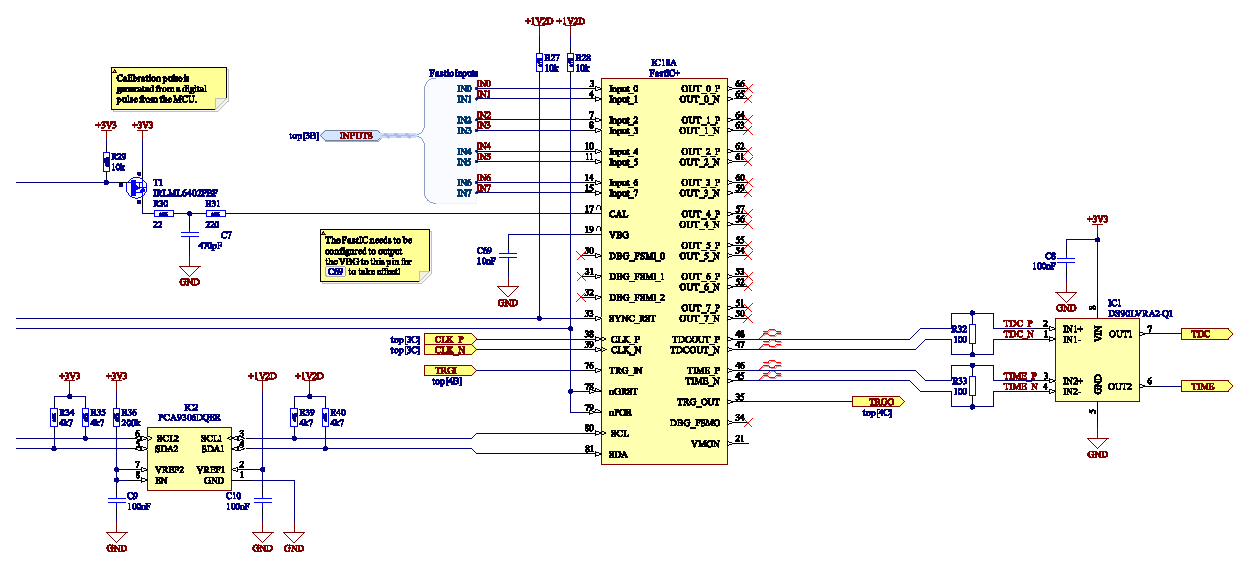
\includegraphics[scale=0.8]{schematic/fastic.eps}
    \caption{Schematic of the FastIC+}
    \label{fig:fastic}
\end{figure}
\FloatBarrier


%
\subsubsection{I2C communication}
As the FastIC+ voltage domains all run at \SI{1.2}{\volt}, a voltage shifter had to be implemented for communication with the microcontroller over I2C. For this, the PCA9306DQER has been chosen for its miniature X2SON package and sufficent \SI{400}{\kilo\hertz} speed. 
%
\subsubsection{Calibration pulse generator}
The FastIC+ features a \verb|CAL| input pin used for injecting a test pulse into any of the eight input channels. This pin converts the pulse to current with an internal \SI{70}{\ohm} resistor. The usual shape of such a pulse should resemble a real sensor output, thus a decaying exponential with an amplitude of a few milliamperes and length under a microsecond. To create this pulse, a high side switch has been implemented with series resistance to limit the current and parallel capacitance to recreate the decaying exponential. The transistor gate is driven by a quick digital pulse from the microcontroller, whos length can be adjusted to adjust the current pulse width and by some degree also the amplitude. 
%
\subsubsection{Voltage monitoring}
%
The \verb|VMON| pin on the ASIC serves for monitoring of the internal analog tresholds and DAC outputs. Since the microcontrollers internal voltage reference has been selected to run at \SI{1.8}{\volt}, a simple non inverting amplifier has been implemented to amplify the \SI{1.2}{\volt} output to the microcontrollers full-scale range and improve the performance. Because the \verb|VMON| output is used only for treshold monitoring, thus only DC voltages, a slow RC filter has been used to reduce the noise coupled to the analog signal.
%
\FloatBarrier
\begin{figure}[htp!]
    \centering
    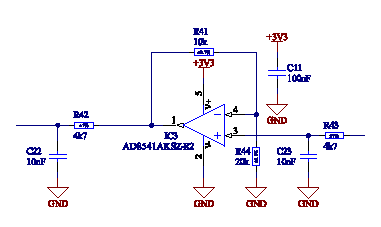
\includegraphics[scale=2]{schematic/fastic_vmon.eps}
    \caption{Schematic of the voltage monitoring amplifier}
    \label{fig:fastic_vmon}
\end{figure}
\FloatBarrier
%
\subsubsection{High speed outputs}
%
The FastIC+ offers multiple high speed SLVS outputs. For each channel, a differential output is present capable of transmitting a pulse whos beginning timestamps the ToA of a photon and length resembles the ToT. However, as the readout uses the data digitalized by the internal TDC, these channels can be left unconnected and disabled in the chip.

The \verb|TIME| output can either be used to generate a digital pulse whenever a pulse is received on any of the channels or can be internally connected to the trigger comparator and used for trigger calibration routine, the latter being used in this case. When the pin is not used for calibration, it should be disabled to reduce any EMI generated by the high speed edges. The \verb|TDCOUT| is the output of the Aurora stream from the transmitter.

Both of the above mentioned pins are converted to a CMOS signal using the DS90LVRA2 dual channel differential line receiver. This receiver has been chosen specifically for its small size, high enough speed but also for its typical propagation delay $t_{pd}$ = \SI{4.4}{\nano\second} to correctly align the data to the sampling clock.

\subsubsection{Trigger input and output}
The trigger inputs (used for externally triggering the ASIC) and outputs (outputting the signal from the internal comparator) have been exposed to the user on two SMA connectors. Termination has been placed on these to mitigate any reflections and ESD protection diodes have been added to protect the chip from ESD events. It's important to note that the ESD diodes add capacitance to the trigger lines, thus degrading (slowing) the trigger edge and introducing a slight delay in the trigger. This either needs to be accounted for when using the readout or the diodes need to be left unassembled at the expense of worse ESD immunity. 
%
\FloatBarrier
\begin{figure}[htp!]
    \centering
    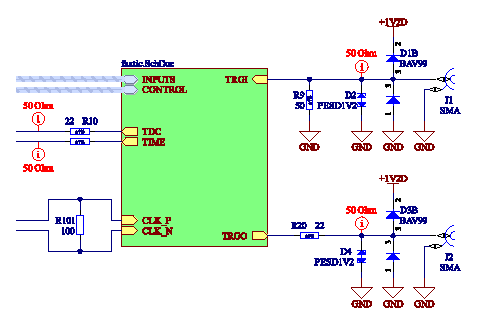
\includegraphics[scale=1.8]{schematic/fastic_top.eps}
    \caption{Schematic of the FastIC+ trigger circuitry}
    \label{fig:fastic_triggers}
\end{figure}
\FloatBarrier

\subsection{USB}
To supply power to the device and handle communication with the host computer, a USB type C connector has been used.
\FloatBarrier
\begin{figure}[htp!]
    \centering
    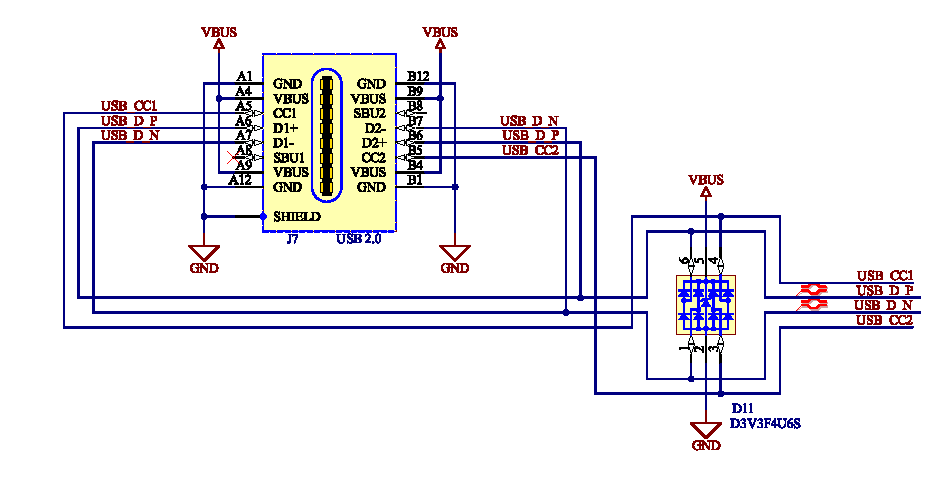
\includegraphics[scale=.9]{schematic/usb_con.eps}
    \caption{Schematic of the USB connector with ESD protection}
    \label{fig:fastic_triggers}
\end{figure}
\FloatBarrier
\subsubsection{External PHY}
Because the combined data rate of the FastIC+ chips of \SI{160}{\mega\bit\per\second} exceeds the USB 1.1 specification, a USB 2.0 (High Speed) was implemented, supporting up to \SI{480}{\mega\bit\per\second} throughput. Unfortunately, the used microcontroller does not integrate the USB 2.0 PHY directly. Instead, it only integrates the necessary logic and interfaces with an external PHY via the ULPI interface. 


A USB3320 interface was chosen as it is well supported by the microcontroller and widely used in countless designs. A \SI{48}{\mega\hertz} crystal oscillator has been used as the external reference clock required for the device to operate. Different crystal frequency selection has been made possible with \SI{0}{\ohm} resistor jumpers. The ULPI connections have been series terminated, to suppress any possible reflections caused by poor impedance matching. 
\FloatBarrier
\begin{figure}[htp!]
    \centering
    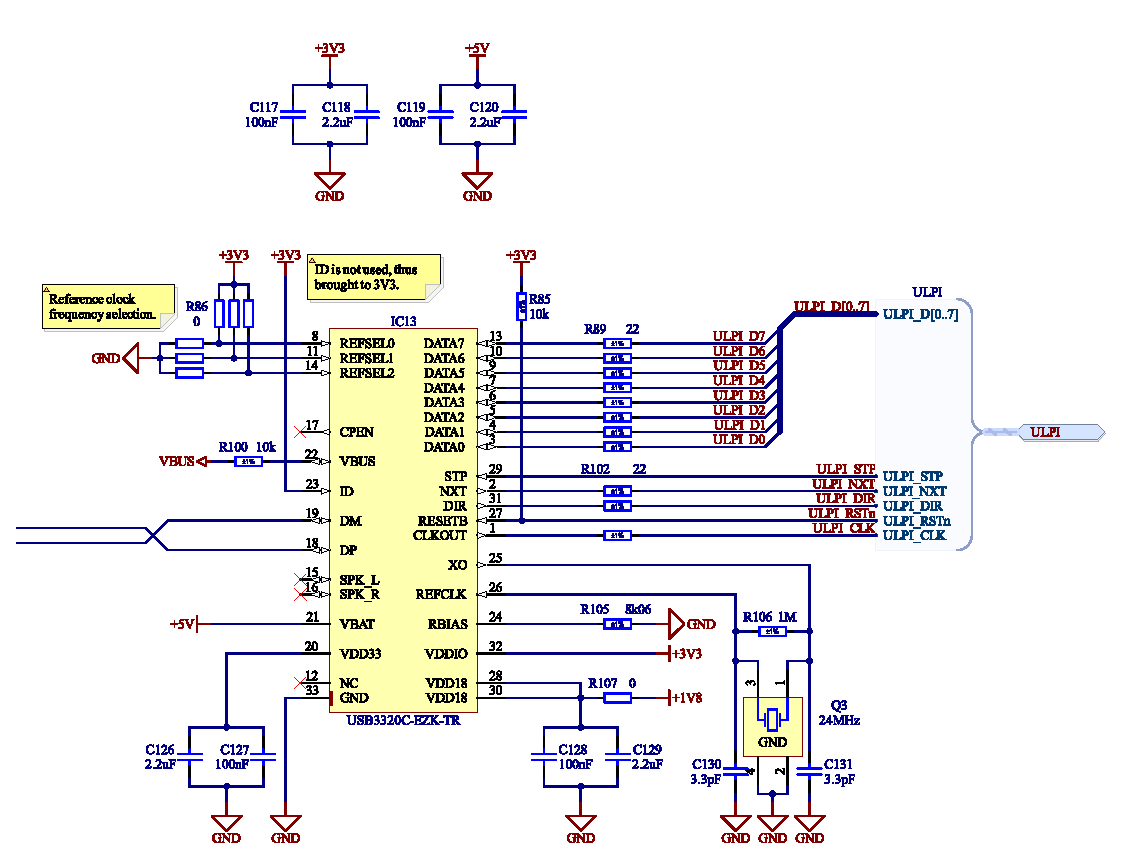
\includegraphics[scale=.8]{schematic/usb.eps}
    \caption{Schematic of the USB}
    \label{fig:fastic_triggers}
\end{figure}
\FloatBarrier
\subsubsection{Power Delivery}
A FUSB302 chip was added to allow for power limit negotiation with a UCPD capable power source. The chip handles all the necessary signaling and communicates with the MCU via a I2C interface. Optional \SI{5.1}{\kilo\ohm} resistors have been added to passively negotiate the highest power limit, if it would be decided to omit the power delivery functionality and not assemble the FUSB302.
\FloatBarrier
\begin{figure}[htp!]
    \centering
    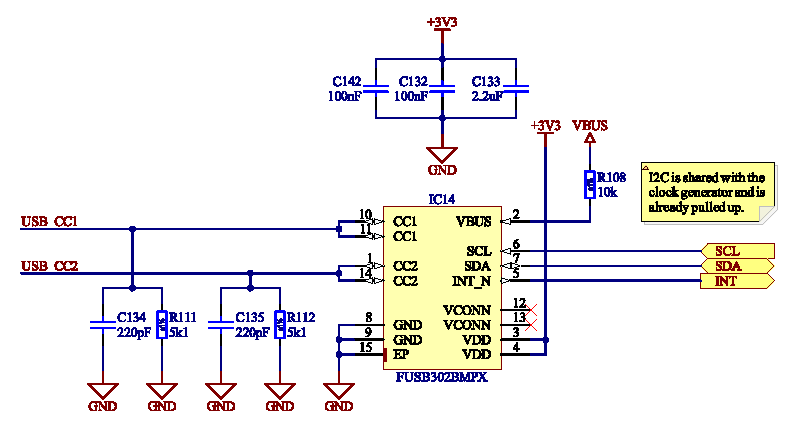
\includegraphics[scale=1.2]{schematic/ucpd.eps}
    \caption{Schematic of the USB}
    \label{fig:fastic_triggers}
\end{figure}
\FloatBarrier
\subsection{Clock generation}
For generating the \SI{40}{\mega\hertz} reference clock for both of the FastIC+ chips and the \SI{80}{\mega\hertz} sampling clock for the SPI peripherals, a SI5340 has been used. It is a four output clock generator with \SI{90}{\femto\second} RMS jitter, supporting both CMOS and differential output. Additionally, each output can be powered by an independent power supply allowing for mixing the \SI{3.3}{\volt} CMOS signals for the microcontroller and \SI{1.8}{\volt} LVDS signals for the FastIC+. A \SI{48}{\mega\hertz} crystal oscillator has been used as the reference clock. The chip features both I2C and SPI interface for configuration. The I2C was selected to be used in this design.
\FloatBarrier
\begin{figure}[htp!]
    \centering
    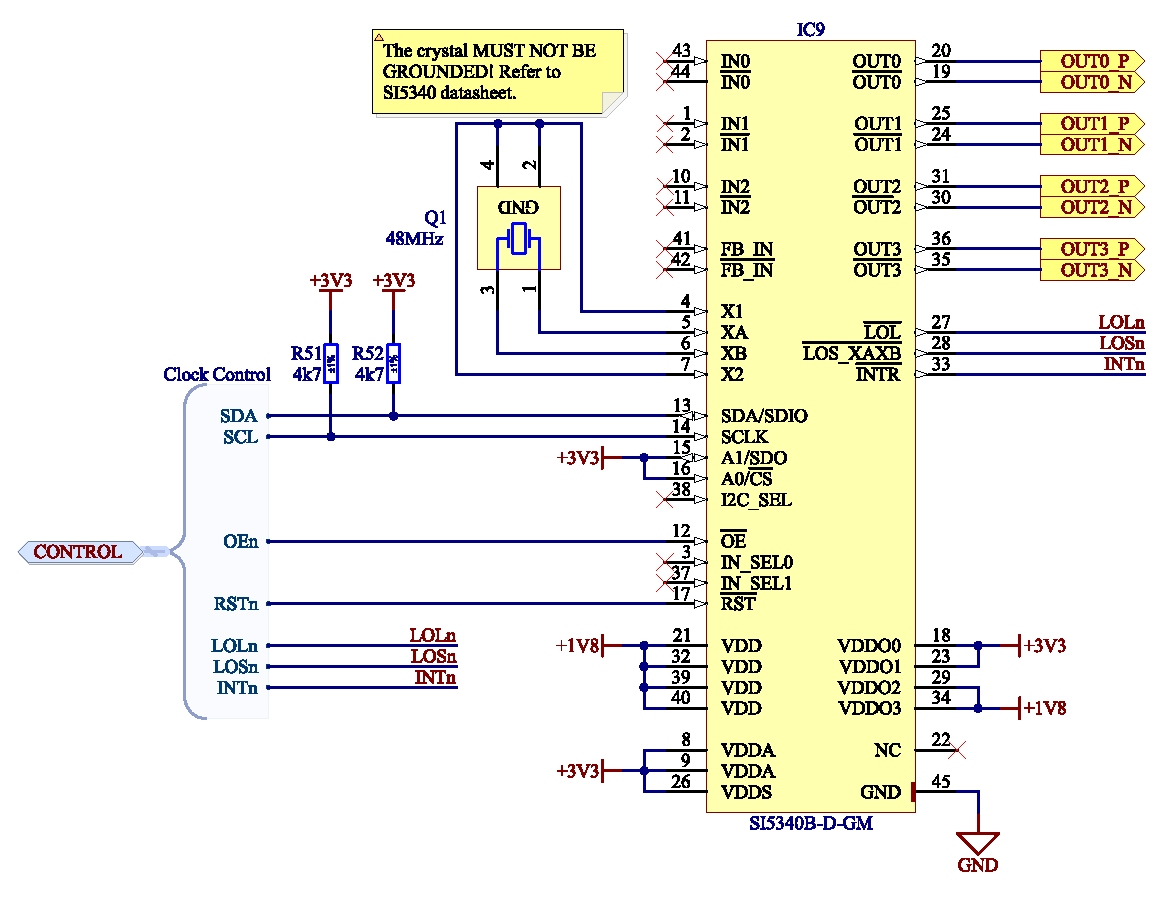
\includegraphics[scale=0.8]{schematic/clock.eps}
    \caption{Schematic of the clock generator}
    \label{fig:fastic_triggers}
\end{figure}
\FloatBarrier

Unfortunately, the FastIC+ implements SLVS instead of LVDS, which uses voltages down to \SI{1.2}{\volt}, not supported by the generator. Because of this, a divider on the differential had to be implemented. This circuit was provided by the chip designers themself and has been proven to work reliably, thus is not explained in detail in this document. 
\FloatBarrier
\begin{figure}[htp!]
    \centering
    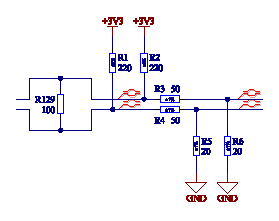
\includegraphics[scale=2]{schematic/slvs.eps}
    \caption{Divider for the LVDS to SLVS conversion}
    \label{fig:fastic_triggers}
\end{figure}
\FloatBarrier

\subsection{High Voltage}
All the usual sensors like SiPMs, PMTs or MCPs need high voltage biasing for their function. To eliminate the need for an external HV supply, an internal one has been implemented using the LT3571. This DC/DC converter, intended for biasing of avalanche photodiodes, is capable of generating up to \SI{70}{\volt} \SI{2}{\milli\ampere} output from a low voltage input. It fully integrates the power switch and regulation along with soft-start and variable switching frequency. 

\FloatBarrier
\begin{figure}[htp!]
    \centering
    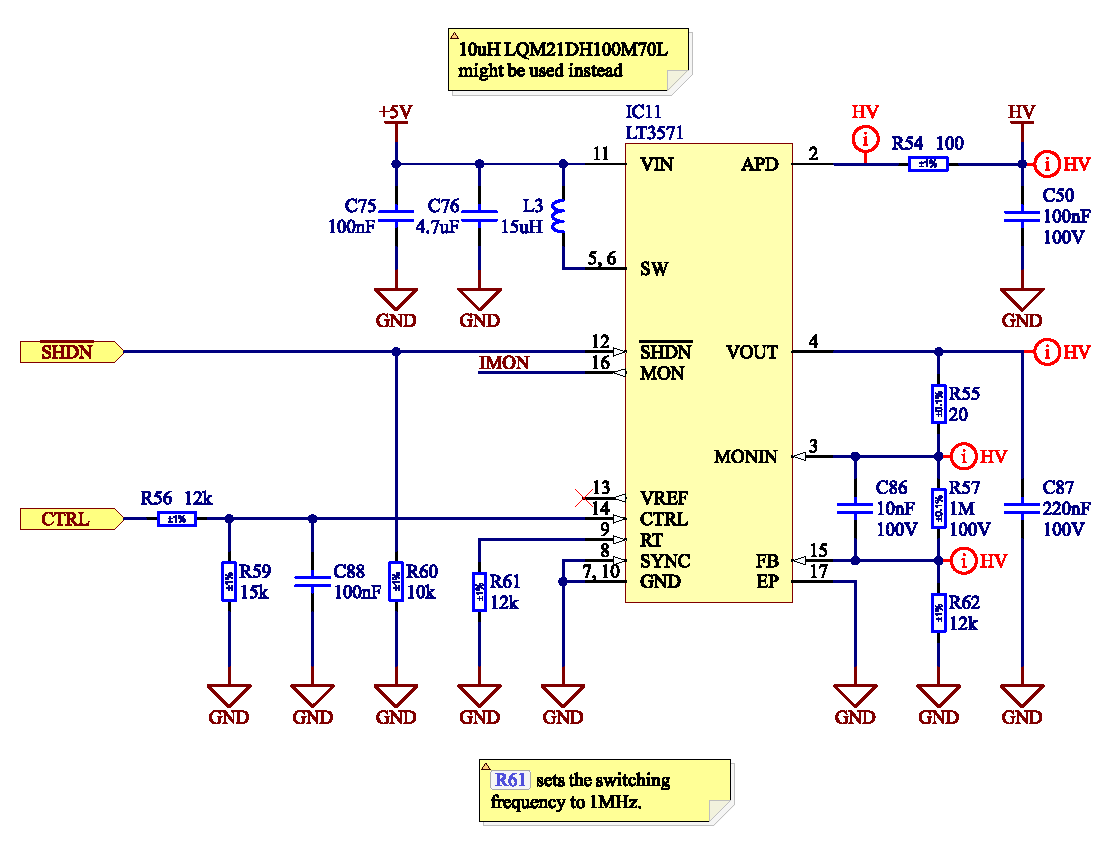
\includegraphics[scale=.8]{schematic/hv.eps}
    \caption{High voltage power supply schematic}
    \label{fig:fastic_triggers}
\end{figure}
\FloatBarrier

A \verb|CTRL| input is available for adjusting the output with a control voltage. This reference is generated by the MCU DAC and divided by a voltage divider to a suitable \SI{0}{V} -  \SI{1}{V} range. 

To allow for closed loop control with the microcontroller, the output voltage on the APD pin is monitored via a suitable voltage divider with an operational amplifier buffer. For current monitoring, the LT3571 offers the \verb|IMON| pin outputting a current proportional to the one out of the \verb|APD| pin. This current is than converted to voltage with a \SI{1}{\kilo\ohm} shunt and buffered with an operational amplifier. 

\FloatBarrier
\begin{figure}[htp!]
    \centering
    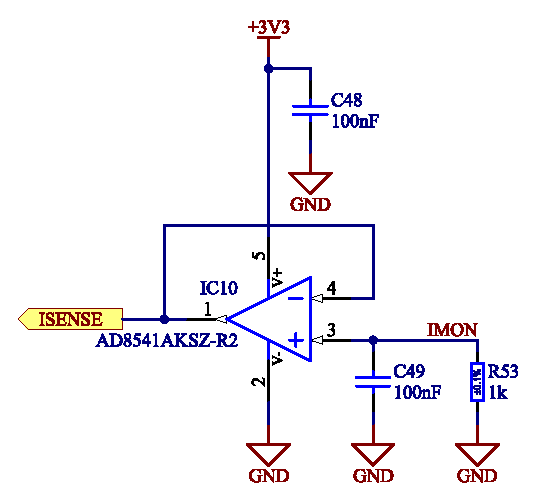
\includegraphics[scale=.8]{schematic/hv_isense.eps}
    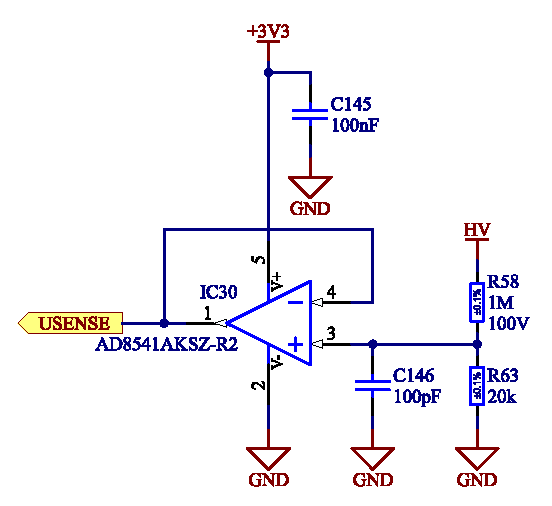
\includegraphics[scale=.8]{schematic/hv_usense.eps}
    \caption{Sensing of the high voltage and current}
    \label{fig:fastic_triggers}
\end{figure}
\FloatBarrier

\subsection{Power}
A DC/DC converter has been implemented to efficiently lower the \SI{5}{\volt} input voltage to the \SI{3.3}{\volt} used by the microcontroller. The \SI{3.3}{\volt} for the analog domain has been generated with a low ripple LDO. The \SI{1.8}{\volt} domain for the USB interface has been derived from the \SI{3.3}{\volt} using an LDO aswell, as the low power consumption will not cause too much of a power loss. 

\FloatBarrier
\begin{figure}[htp!]
    \centering
    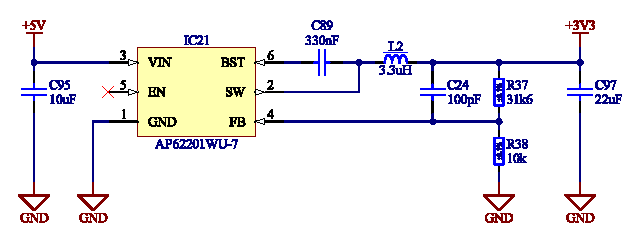
\includegraphics[scale=1]{schematic/power_dcdc.eps}
    \caption{Step down regulator schematic}
    \label{fig:fastic_triggers}
\end{figure}
\FloatBarrier

A power sequencing has been implemented for all the three FastIC+ domains. First, the digital domain supply is activated, followed by the supply for the treshold circuitry and PLL and lastly, the analog domain is supplied. All of these domains are derived from the \SI{3.3}{\volt} using a \SI{1.2}{\volt} LDOs which are sufficient for the low power consumption of the FastIC+ chips.

\FloatBarrier
\begin{figure}[htp!]
    \centering
    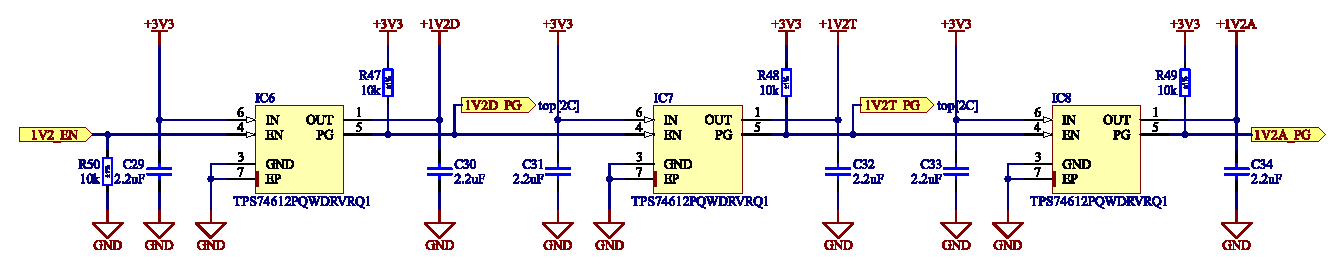
\includegraphics[scale=.7]{schematic/power_fastic.eps}
    \caption{FastIC+ power domain sequencing}
    \label{fig:fastic_triggers}
\end{figure}
\FloatBarrier

\subsection{Connector}
For interfacing with the user board, the \SI{9}{\milli\meter} high version of ERM8-020 has been used for its durability and suitable pin count. This connector carries all the sixteen input channels alongside the high voltage biasing supply. The \SI{3.3}{\volt} supply is also exposed and four pins are dedicated to the user board identification.
\subsubsection{Identification pins}
The identification pins serve as an easy way to assign a four bit ID to a specific user board. This ID can than be used by the software to load a configuration preset defined for the user board. For advanced cases, the pins ID0 and ID1 are used as I2C communication lines. A compatible EEPROM can than be assembled on the user board, saving the full configuration on the user board itself, as well as additional data like name. If the I2C interface is to be used, all the ID pins need to be pulled up high by a suitable resistor. At least one of the ID pins has to be high at all times, this means that an ID of \verb|0b0000| is not allowed and in this case, the readout will not recognize a valid user board. 
%
\section{User Board}
The user board has been developed as a template for the users to get easily started with the readout system. It contains a matrix of 4 $\times$ 4 SiPM sensors as well as an EEPROM for storing the board configuration. The \SI{9}{\milli\meter} high ERF8-020 connector has been chosen for the user board to match the counterpart present on the readout and allow enough clearance between the assembled readout board and user board.

\subsection{Sensors}
The footprint for a typical generic THT SiMPs has been implemented on the board. Each SiPM is powered from the HV plane and the input is filtered with a dual RC low pass to eliminate a possibility of cross triggering of the sensors. 

\FloatBarrier
\begin{figure}[htp!]
    \centering
    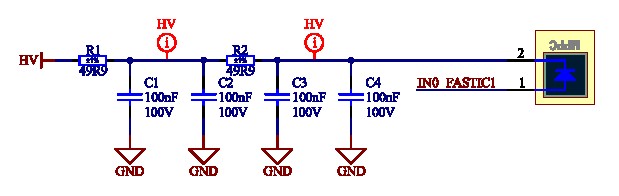
\includegraphics[scale=1.2]{schematic/sipm.eps}
    \label{fig:sipm}
\end{figure}
\FloatBarrier

\subsection{EEPROM}
The 24AA04T-I/OT \SI{4}{\kilo\bit} EEPROM has been used on the user board for the configuration storage. It has been selected for the low price and sufficient capacity. 



\newpage
\section{Summary}
The two concepts described above were designed and manufactured keeping in mind the required performance. The final PCBs can be seen on the images bellow. 

\FloatBarrier
\begin{figure}[htp!]
    \centering
    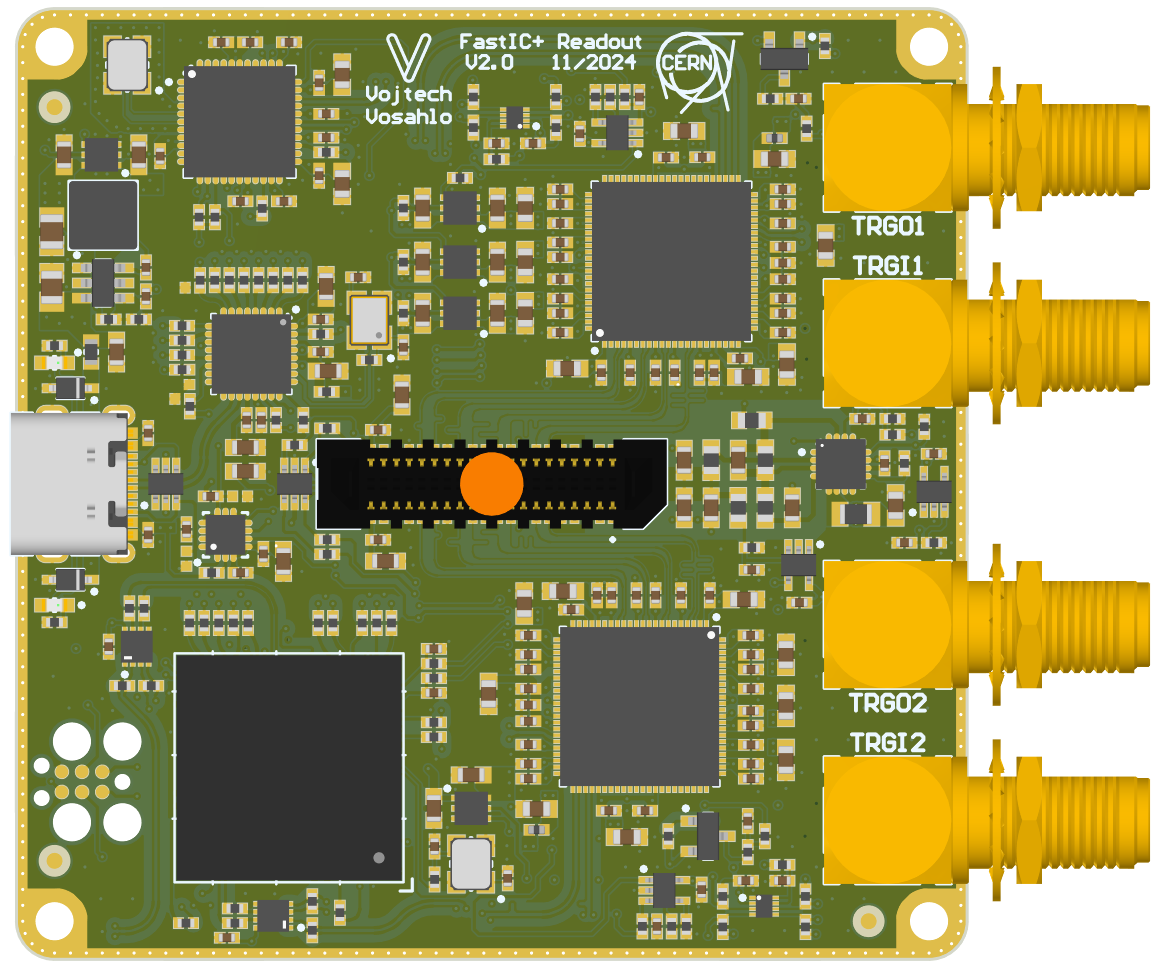
\includegraphics[height=6cm]{readout_3d-top.png}
    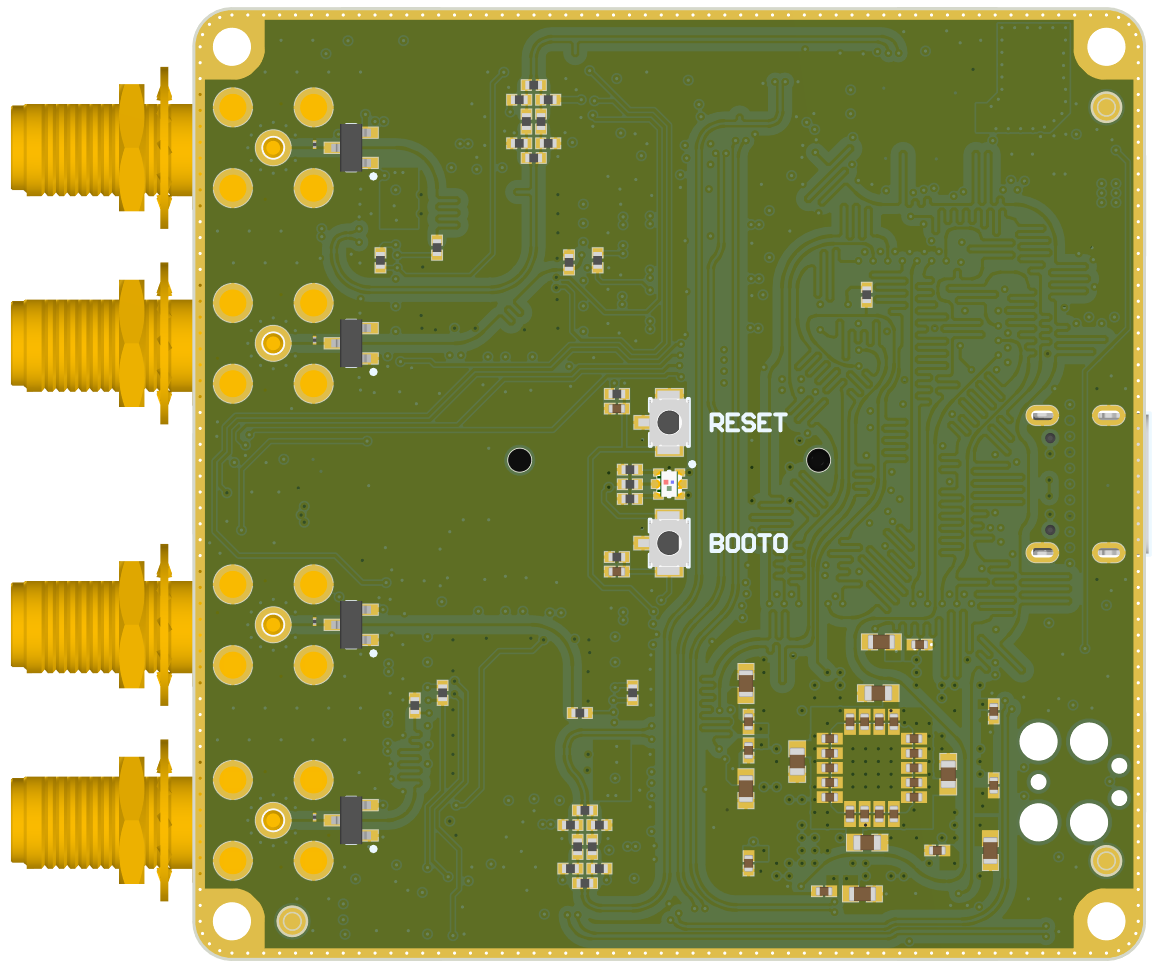
\includegraphics[height=6cm]{readout_3d-bottom.png}
    \caption{The readout PCB}
    \label{fig:readout_3d}
\end{figure}
\FloatBarrier

\FloatBarrier
\begin{figure}[htp!]
    \centering
    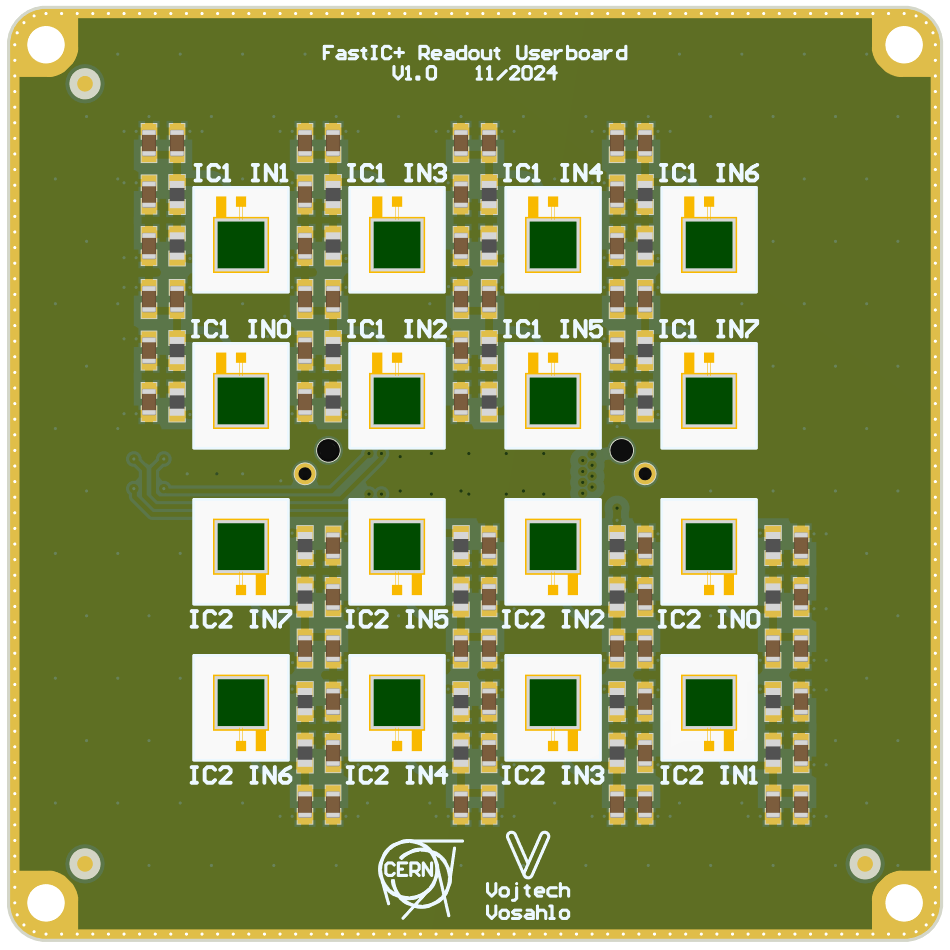
\includegraphics[height=6cm]{userboard_3d-top.png}
    \hspace{2.2cm}
    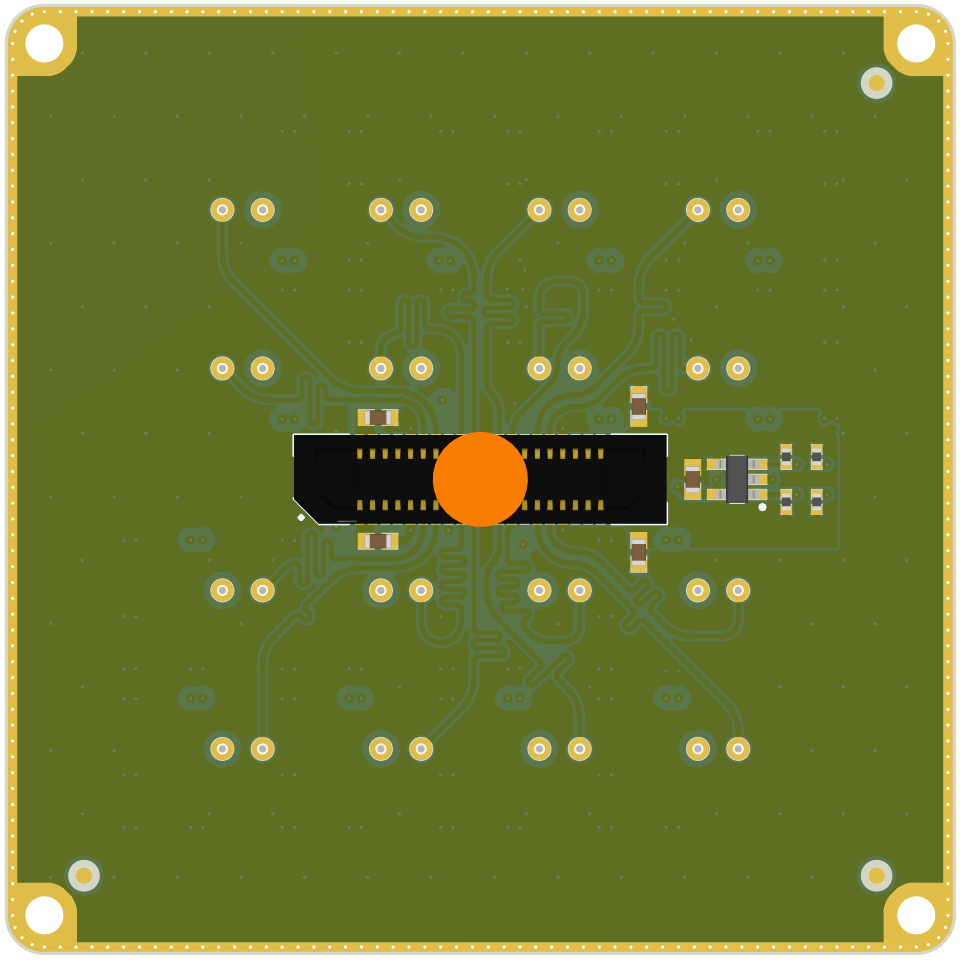
\includegraphics[height=6cm]{userboard_3d-bottom.png}
    \caption{The user board PCB}
    \label{fig:userboard_3d}
\end{figure}
\FloatBarrier

\chapter{Firmware}
A firware in the C++ programming language has been developped for the readout aiming for best performance and reliable functionality. 
\section{USB}
The TinyUSB library has been used for implementing the USB stack on the device. It is an open-source cross-platform USB stack for embedded systems, designed to be memory-safe with no dynamic allocation and thread-safe. It provides support for both Host and Device roles and implements all the common usb classes such as CDC, HID, DFU, Vendor specific and others. On the STM32H7 series specifically, it is capable of working with the ULPI PHY in HS mode and make use of the internal DMA to allow for very high throughput and good latency. All of these specification make it ideal for this application.

Three interfaces have been implemented in order to allow for configuration of the device via human readable protocol, binary protocol and readout of the two data streams.
\subsection{CDC interface}
A Communication Device Class has been implemented on the first interface (endpoints 0x81, 0x82 ans 0x02). This interface emulates a COM port over USB and allows for easy, human-readable interaction with the device. A simple text protocol has been impemented to serve all the required functions of the device. 
\newpage
The following commands have been implemented, where square brackets indicate a choice between the options separated by slash and curly braces indicate value in the specified format:
%
\begin{itemize}
    \item \verb|get readout status| - returns the status of the readout
    \item \verb|get readout uid| - returns a UID of the readout
    \item \verb|get hv enable| - returns the state of the HV supply
\end{itemize}
\begin{verbatim}
set hv enable [true/false]
get hv current
get hv voltage
set hv voltage {float: voltage}
get fastic register [1/2] {hex byte: address}
set fastic register [1/2] {hex byte: address} {hex byte: value}
get fastic voltage [1/2]
get fastic syncreset [1/2]
set fastic syncreset [1/2] [high/low]
set fastic calpulse [1/2] [enable/disable]
get fastic time [1/2]
get fastic aurora [1/2]
set fastic aurora [1/2] [enable/disable]
get userboard status
get userboard uid
get userboard name
set userboard name {string: name}
get userboard writeprotect
set userboard writeprotect [true/false]
get userboard init
set userboard init 
get userboard voltage 
set userboard voltage {float: voltage}
get userboard register [1/2] {hex byte: address}
set userboard register [1/2] {hex byte: address} {hex byte: value}
set userboard tomemory
set userboard frommemory
\end{verbatim}

A detailed description of the commands and their usage is provided in the device user manual.

\subsection{Vendor control}
The USB specification describes a way to communicate with a USB device in a bursty matter by Control Transfers. A control transfer is typically a short random packet, containing up to \SI{64}{\byte} of data, which is delivered to the default endpoint with the best effort delievery (no retransmissions). These packets are, for example, used to control the flow of the CDC interface but can be very easilly adopted to transfer auxilary vendor data and thus allow for binary communication with the device. 

The same commands as in the CDC interface have been implemented using control transfers to allow for easier interactions with the device via software on the PC as the text communication adds unneccessary overhead in thios regard.

A control transfer is started by an eight byte long Setup Packet, which contains the following fields:

\FloatBarrier
\begin{figure}[htpb]
    \begin{center}
        \begin{bytefield}[endianness=little,bitwidth=1em, bitheight=1.2em]{32}
            \bitheader{0,7,8,15,16,31} \\
            \bitbox{8}{\texttt{\footnotesize bmType}} & 
            \bitbox{8}{\texttt{\footnotesize bRequest}} & 
            \bitbox{16}{\texttt{\footnotesize wValue}} \\[3ex]
            \hfill
            \bitheader[lsb=32]{32,47,48,63} \\
            \bitbox{16}{\texttt{\footnotesize wIndex}} & 
            \bitbox{16}{\texttt{\footnotesize wLength}} 
        \end{bytefield}
        \caption{Setup packet structure}
        \label{fig:usb_control_transfer}
    \end{center}
\end{figure}


\verb|bmType| indicates the direction of the communication, the type, in this case a Vendor transfer, and the recipient, in this case a Device. \verb|bRequest| field indicates the request number. The readout text commands have been each mapped to a unique number which is used in this field in the binary communication. \verb|wValue| and \verb|wIndex| allow for other parameters to be passed with the request, in this case parameters such as the index of the FastIC+ chip to work with. If there is more data to be transfered, the \verb|wLength| field is used to specify the length of an additional data packet sent after the Setup Packet.

\subsection{Vendor interfaces}
For transfering the Aurora data stream from the FastIC+ chips to the computer, two vendor interfaces have been implemented, one for each FastIC+ chip. The sampled bitstream is transfered using Bulk Transfers over these two interfaces. 

\section{Clock generation}
The configuration for the Si5340 clock synthetizer was generated using the Clock Builder application provided by Skyworks. This software generates a register map as a C/C++ array that is later parsed by the software and the configuration is applied to the synthetizer over I2C.

\section{HV power supply}
For controlling the HV power supply, a DAC peripheral has been used to provide the control voltage. Two channels of an ADC peripheral with 256 times oversampling, resulting in a \SI{1000}{\hertz} sample rate, were than used to acquire feedback for voltage and current monitoring. 

\subsection{PID controller}
A closed control loop was implemented, using the ADC inputs and DAC output called a PID controller. This controller calculates the DAC value in order to minimize the difference between a required output voltage and a feedback from the ADC. On every cycle, which takes place after the ADCs finished sampling, an error value $e$ is calculated, which represents the difference between the setpoint and the measured voltage. The error is than integrated into variable $I$ and a derivation of the measured value is calculated, denoted $D$. In the end, a corrective output setting is calculated, to compensate for possible error, using the following equation:

\begin{equation}
    O = K_P \cdot e + K_I \cdot I + K_D \cdot D
\end{equation}
where $O$ is the output value and $K_P$, $K_I$ and $K_D$ are the progressive, integral and derivative constants respectively.

The afformentioned constants can either be determined analytically after modelling the control loops transfer function, heuristically, for example by the Ziegler-Nichols method or manually which was chosen in this case. First, the proportional constant was set to a value that would bring the output close to the desired value while not causing any oscilations. Than, the integral part was increased to minimize the steady state error but kept safe bellow any oscillation treshold. Overshoots and undershoots of the regulator were examined with every change. Finally, the derivative part was added to improve the dynamic response and the performance was tested. The values of $K_P = 150$, $K_I = 3$ and $K_D = 10$ were fond to be suitable for the regulator.
\section{FastIC+}
Both of the FastIC+ chips are mainly controlled over the I2C interface. Only a very basic configuration is done by the software, setting the propper clock dividers to be able to receive the Aurora stream. Rest of the settings are left for the user to modify, as the registers of the FastIC+ can be accessed directly over the communication interface and most of them need to be tuned for a specific application of the readout.

\subsection{Aurora stream}
The Aurora stream is continuously sampled by an SPI interface on the rising edge of the sampling clock. The SPI interface buffers the received bytes in its internal FIFO until a DMA peripheral, configured in double-buffer circular mode, transfers the data to a buffer. In the double buffer mode, the programmer provides the DMA wit two separate buffers. The DMA is than configured to switch back and forth between the buffers every time one of them is full. This allows the rest of the code to transfer data from one of the buffers while the other one is being filled, not causing any bit drops. 

\subsection{Pulse injection}

The pulse injection circuit is fed by a fast timer output. The width of the timer pulse directly influences the width and amplitude of the generated pulse which is used for testing the frontends. The size of this pulse has been fixed and the pulses are generated with a period of \SI{100}{\hertz}. 
\newpage
\section{Userboard}

The userboard detection is achieved with the four exposed GPIO pins. When a command, such as \verb|get userboard status| tries to access the userboard, the short ID is first obtained. If the short ID equals \verb|0b1111|, the pins are switched into a I2C mode and the microcontroller checks if a configuration header is present in the EEPROM. 

The following structure of a configuration header has been implemented:

\FloatBarrier
\begin{figure}[tph!]
    \begin{center}
        \begin{bytefield}[endianness=little,bitwidth=1em, bitheight=1.2em]{32}
            \bitheader{0,1,2,3,4,5,6,7,8,9,10,11,12,13,14,15,16,17,18,19,20,21,22,23,24,25,26,27,28,29,30,31} \\
            \bitbox[lrt]{32}{}\\
            \bitbox[lr]{32}{\texttt{\footnotesize UID}}\\
            \bitbox[lr]{32}{\texttt{\footnotesize (128 bits)}}\\
            \bitbox[lrb]{32}{}\\
            \bitbox[lbr]{32}{\texttt{\footnotesize WRITE CYCLES}}\\
            \bitbox[lrb]{1}{\texttt{\tiny WP}} & \bitbox[lrb]{1}{\texttt{\tiny UI}} & \bitbox[lrb]{1}{\texttt{\tiny NI}} & \bitbox[lrb]{1}{\texttt{\tiny VI}} & \bitbox[lrb]{1}{\texttt{\tiny F1I}} & \bitbox[lrb]{1}{\texttt{\tiny F2I}} & \bitbox[lrb]{2}{\texttt{\tiny RES}} & \bitbox[lr]{24}{}\\
            \bitbox[lr]{32}{\texttt{\footnotesize RESERVERD}}\\
            \bitbox[lr]{32}{\texttt{\footnotesize (120 bits)}}\\
            \bitbox[lr]{32}{}\\
            \bitbox[lrt]{32}{} \\
            \bitbox[lr]{32}{}\\
            \bitbox[lr]{32}{}\\
            \bitbox[lr]{32}{}\\
            \bitbox[lr]{32}{}\\
            \bitbox[lr]{32}{}\\
            \bitbox[lr]{32}{}\\
            \bitbox[lr]{32}{\texttt{\footnotesize NAME}}\\
            \bitbox[lr]{32}{\texttt{\footnotesize (512 bits)}}\\
            \bitbox[lr]{32}{}\\
            \bitbox[lr]{32}{}\\
            \bitbox[lr]{32}{}\\
            \bitbox[lr]{32}{}\\
            \bitbox[lr]{32}{}\\
            \bitbox[lr]{32}{}\\
            \bitbox[lrb]{32}{} \\
            \bitbox[lrb]{32}{\texttt{\footnotesize VOLTAGE}} 
           
        \end{bytefield}
    \end{center}
    \caption{EEPROM configuration header structure}
    \label{fig:config_header}
\end{figure}
\FloatBarrier

where \verb|UID| is a unique ID generated on first initialization of the userboard, \verb|WRITE CYCLES| stores the number of times that the EEPROM has been written. \verb|WP| is a write protect bit and the \verb|UI|, \verb|NI|, \verb|VI|, \verb|F1I|, \verb|F2I| signal if the UID, name, voltage value, FastIC+ 1 and FastIC+ 2 registers have been initialized respectively. \verb|NAME| contains up to 64 character user name and \verb|VOLTAGE| is a floating point value that stores the high voltage preset of a given userboard.


\chapter{Software}
A simple Python-based software application was developed to handle basic user tasks. Python was chosen for its simplicity, ease of use, and widespread adoption within the scientific community. However, this choice comes with certain drawbacks, such as reduced performance, which becomes noticeable when processing large amounts of data, such as binary streams. To address this, efforts were made to optimize the code for speed wherever possible.

The first component of the software is a library of functions for communicating with the device via vendor control transfers and for reading FastIC+ data streams into binary files. The `pyusb` library was utilized for both vendor control transfers and bulk data transfers.

The second component is a library designed to process the captured data. This library handles synchronization, decoding, and parsing of the data, ultimately outputting FastIC+ packets as objects. It aligns the bitstream using detected Aurora synchronization preambles, reads the block data, descrambles it, and assembles it into packets.

Finally, these two components were integrated into a simple example script. This script configures the FastIC+ parameters, sets up the HV bias, captures a sample data stream, and decodes it. Additional functionality, such as the comparator calibration procedure, remains to be implemented. These tasks are left either to the users or to the FastIC+ researchers, who, with their in-depth knowledge of the chip, can provide the most efficient implementations.




\clearpage
\FloatBarrier
\printbibliography

\end{document}